\section{Evaluation}
\label{sec:evaluation}

\subsection{Sample Successorships Application}

In our previous project, we created a web application using the presentation framework \textit{Reveal.js}~\footnote{https://github.com/hakimel/reveal.js/, accessed 2019-04-17} to present Successorships to graduate students of the computer science department of the University of British Columbia.
The application used the Successorships API that made use of the Zeroconf protocols based on FlyWeb.
Obviously, the presenters had to have a Mac computer and a dedicated old version of Firefox Developer Edition with the FlyWeb addon installed to be able to present.
Moreover, the previously mentioned performance problems were clearly visible, with recovery of the system from intentionally injected faults taking over 20 seconds at times.
In a similar fashion, we presented Zeroties to an audience of graduate students at the same university.
The presentation technicalities remained the same, except that the API usage within Successorships was changed from FlyWeb to Zeroties.
To demonstrate this new independence of Firefox, the presentation was performed on Google Chrome.
A significant decrease in time-to-recovery after failure could clearly be observed with the system recovering in very few seconds.

\subsection{Empirical Evaluation}

We reproduced the performance measurements from the previous paper in order to analyze changes in performance from the old to the new version of Successorships.
We collected traces for system recovery for the following scenario, first with the old FlyWeb-based version on Mozilla Firefox, and then with the new Zeroties-based version on Google Chrome:
\begin{itemize}
\item One node starts the app and becomes the server.
\item 5 nodes start the app and become clients.
\item The server broadcasts 7 messages to all clients.
\item The server dies and the next successor becomes the server.
\item The other 4 clients become clients to the new server.
\end{itemize}

This process was first repeated until only the last node remained and became the server.
Afterwards, 5 more nodes started the application and became clients of that last remaining node from the last run that was now serving.
The process was then repeated once more until the last node was finally terminated.
In total, this process therefore involved 9 recoveries from server failures.
The scenario was performed on one machine where one node constituted one browser window.
While we acknowledge that a multi-machine experiment would have been more representative, we argue that for the analysis of performance changes between the two version this infrastructural change would not be significant.

Table~\ref{tbl:eval:time-to-recovery} shows the time to recovery in seconds for the described scenario with FlyWeb and Zeroties.
It is visible, that the Zeroties version recovered from failures nearly 10 times faster with little variation.
Figure~\ref{fig:eval:server-recovery} compares the cumulative distribution between the two versions that confirms this finding.

\begin{table}
    \caption{Time-to-recovery in seconds with FlyWeb and Zeroties}
    \label{tbl:eval:time-to-recovery}
    \centering
    \begin{small}
    \begin{tabular}{C{1cm}|C{2.5cm}|C{2.5cm}}
    \hline
    \bfseries Failure \# & \bfseries FlyWeb & \bfseries Zeroties \\
    \hline
1 & 15.554 & 1.817 \\
2 & 15.05 & 1.607 \\
3 & 13.183 & 1.701 \\
4 & 13.07 & 1.659 \\
5 & 14.836 & 1.795 \\
6 & 10.652 & 1.726 \\
7 & 11.32 & 1.244 \\
8 & 11.212 & 1.138 \\
9 & 11.473 & 1.269 \\
    \hline
    \end{tabular}
    \end{small}
\end{table}

\begin{figure}[h]
    \centering
    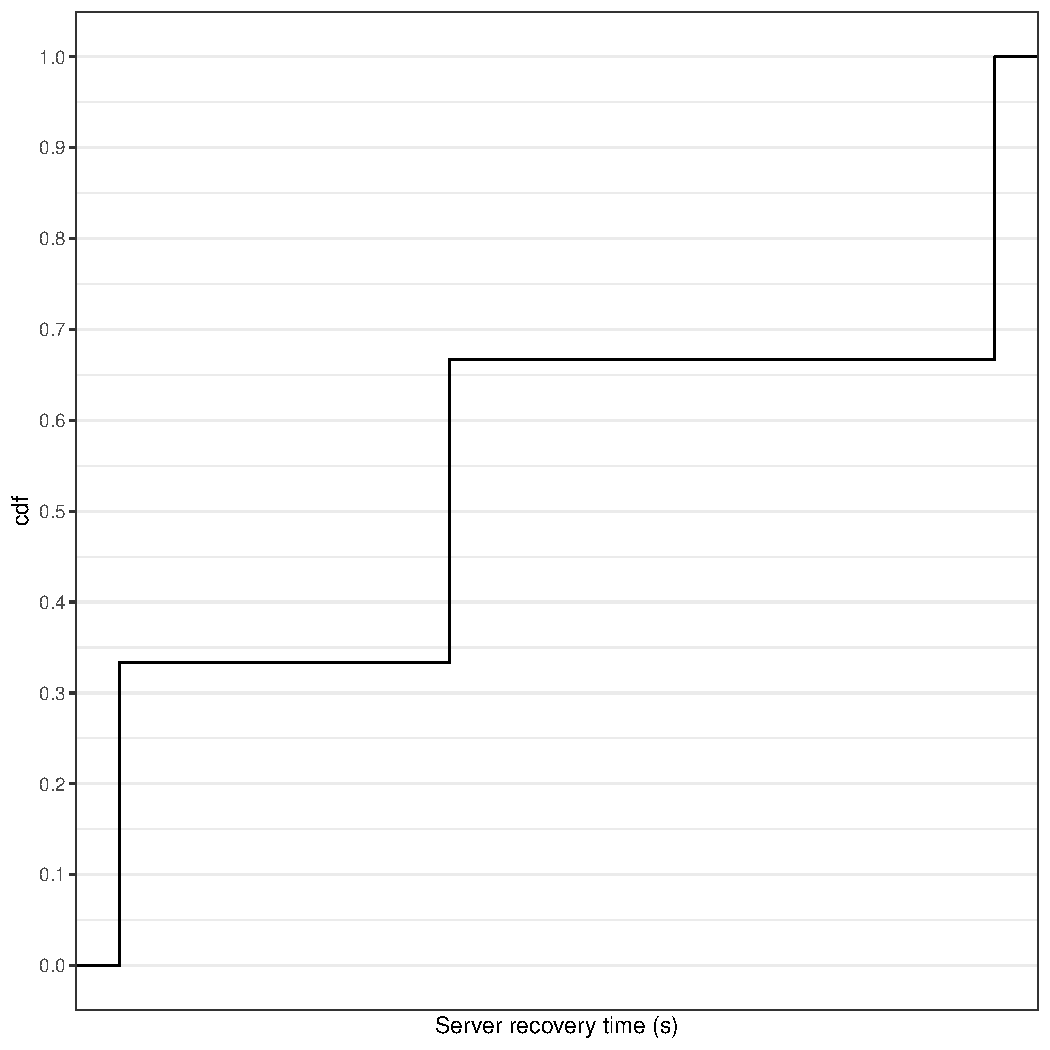
\includegraphics[keepaspectratio,width=\columnwidth]{server-recovery}
    \caption{Comparison of CDFs for server discovery between FlyWeb-based and Zeroties-based versions of Successorships.}
    \label{fig:eval:server-recovery}
\end{figure}